\chapter{Stokes Equation}
\label{cha:stokes-equation}

\section{Problem Overview}
\label{sec:problem-formulation}

A fundamental problem in Solid Earth Sciences in the solution of
Stokes equation for the incompressible creeping flow of a highly
viscous fluid.
\begin{align}
-\div\eta(\grad\vec{v} + \grad\vec{v}^{T}) + \grad p &= \vec{f}\\ 
\div \vec{v} = 0 & 
\end{align}
where $\vec{v}$ is the fluid velocity field,  $p$ is the pressure
which acts to enforce the conpressibility constraint and $\eta$ is the
fluid viscosity.

Computationally and mathematically, Stokes Equation, particularly for
non-constant viscosity, requires somewhat more care to solve than
Poisson's equation in Chapter \ref{cha:poiss-equat-unit}.  To begin
with,   Stokes is a coupled system of PDE's for $\vec{u} =
(\vec{v},p)$ which in finite elements we can capture by describing
$\vec{u}$ as a mixed-element on a mixed Finite element Function space.
The proper choice of elements for $\vec{v}$ and $p$ is critical for
stability and solution of this problem.  Elman et
al. \cite{elman_finite_2005}  provide a good discussion of the issues
for the isoviscous case and \cite{may_preconditioned_2008} provides
important extensions and tests of a large range of iterative solvers
for the variable viscosity case. 

Here we will just illustrate the basic isoviscous problem with a range
of direct and iterative solvers that highlight the Fieldsplit block
preconditioners in PETSc \cite{brown_composable_2012} and their
implementation in \TF{}.  While the computational choices required to
solve Stokes efficiently and accurately are considerably more delicate
than Poisson,  we will demonstrate that setting the problem up in
\TF{} is a straightforward extension of the the problems in Chapter
\ref{cha:poiss-equat-unit}. 

\subsection{Variational forms}
\label{sec:variational-forms}

For this tutorial, we will use a stable ``Taylor-Hood'' element where
velocity is assumed to be a vector valued function with each component
a piecewise quadratic function (i.e.\ for a 2-D problem on triangles
$\vec{v}\in [P_{2}\times P_{2}]$) while the pressure is piecewise
linear ($p\in P_{1}$) such that the entire system $\vec{u}\in \fspace
= [[P_{2}\times P_{2}]\times P_{1}]$.  The variational form of the
(possibly) non-linear problem can be written
\begin{quote}
  \fbox{\parbox{.9\textwidth}{Find $\vec{u}\in \fspace$ such that
      \begin{equation}
         F(\vec{u};\vec{u}_{t}) =0 
      \end{equation}
  for all test functions $\vec{u}_{t}=(\vec{v}_{t},p_{t}) \in\fspace$.}}
\end{quote}
 where $F(\vec{u};\vec{u}_{t}) = F_{\vec{v}} + F_{p}$ and (after some
 algebra and integration by parts)
\begin{align}
         F_{\vec{v}} =  & \int_\Omega \left[\dot{\epsilon}(\vec{v}_{t}):
             2\eta \dot{\epsilon}(\vec{v}_{i}) -
             p_{i}\div\vec{v}_t  - \vec{v}_{t} \cdot\vec{f} \right]d\vec{x}  \\
 F_{p} =& \int_\Omega p_t\div\vec{v}_{i} d\vec{x}
\end{align}
Here
\begin{equation}
  \label{eq:19}
  \dot{\epsilon}(\vec{v}) = \frac{1}{2}
  \left(
\grad\vec{v} + \grad\vec{v}^{T}
  \right)
\end{equation} is the strain-rate tensor (i.e. the symmetric part of
deformation tensor $\grad\vec{v}$).   

The weak form of the residual in UFL looks quite similar
\begin{lstlisting}[style=UFL]
F_v = (inner(sym(grad(v_t)),2.*eta*sym(grad(v_i)))
    - p_i*div(v_t) - inner(v_t,f)*dx  
F_p = p_t*div(v_i)*dx 

F =  F_v + F_p 
\end{lstlisting}
and the Jacobian
\begin{lstlisting}[style=UFL]
  J = derivative(F,u_i,u_a)
\end{lstlisting}
assembles into the $2\times2$ block system
\begin{equation}
  \label{eq:20}
  J =
  \left[
    \begin{array}{cc}
      K & G \\
      G^{T} & 0\\
    \end{array}
  \right]
\end{equation}

The discrete problem Eq. (\ref{eq:20}),  is the classic Stokes
saddle-point system and can be challenging to solve (and is singular
for many simple boundary conditions).  Here we will just scratch the
surface with a simplied MMS solution and some basic solution
strategies taken from \cite{elman_finite_2005}.  To fully specify the problem we need boundary conditions and a
forcing function $\vec{f}$. Elman et. all \cite{elman_finite_2005} provides  the
2-d manufactured solution 
\begin{align}
  \vec{v}_{x}(x,y) =& 20xy^{3} \nonumber \\
  \vec{v}_{y}(x,y) =& 5(x^{4} + y^{4})  \\
   p(x,y) =& 60x^{2}y - 20y^{3} \nonumber \\
   \vec{f}(x,y) =& \vec{0} \nonumber 
\end{align}
on the domain  $\Omega=[-1,1]\times[-1,1]$ with dirichlet boundary conditions on velocity interpolated from the
analytic solution.  Note: the discrete problem with all dirichlet
conditions on velocity is singular (with a trivial constant null space
for the pressure) and some care needs to be taken with both direct and
iterative solvers to solve this problem accurately.

\section{Solution using \TF}
\label{sec:solution-using-tf}

However, setting this problem up in \TF{} is not
much more difficult than solving the scalar Poisson equation.  The
principal changes from the mms problem \texttt{poisson.tfml} are
\begin{itemize}
\setlength{\itemsep}{0em}
\item The system now includes two fields for $\vec{v}$ and $p$
\item The field Velocity, is now vector valued and should be in $P_{2}$
\item The field Pressure is a scalar in $P_{1}$ with no Boundary
  conditions and a constant null space.
\item Each of the fields will require diagnostics, IC's and BC's
\item The forcing term and boundary conditions just need to be made
  consistent for this MMS problem
\item The non-linear residual needs to change to the above UFL
\end{itemize}

A fully worked out \texttt{tfml} file for this problem using a direct
solver along with a script to perform a basic convergence test can be
found in \texttt{\$TF\_HOME/tutorials/stokes/isoviscous/stokes.tfml}.
The solution should look like
\begin{figure}[htbp!]
  \centering
  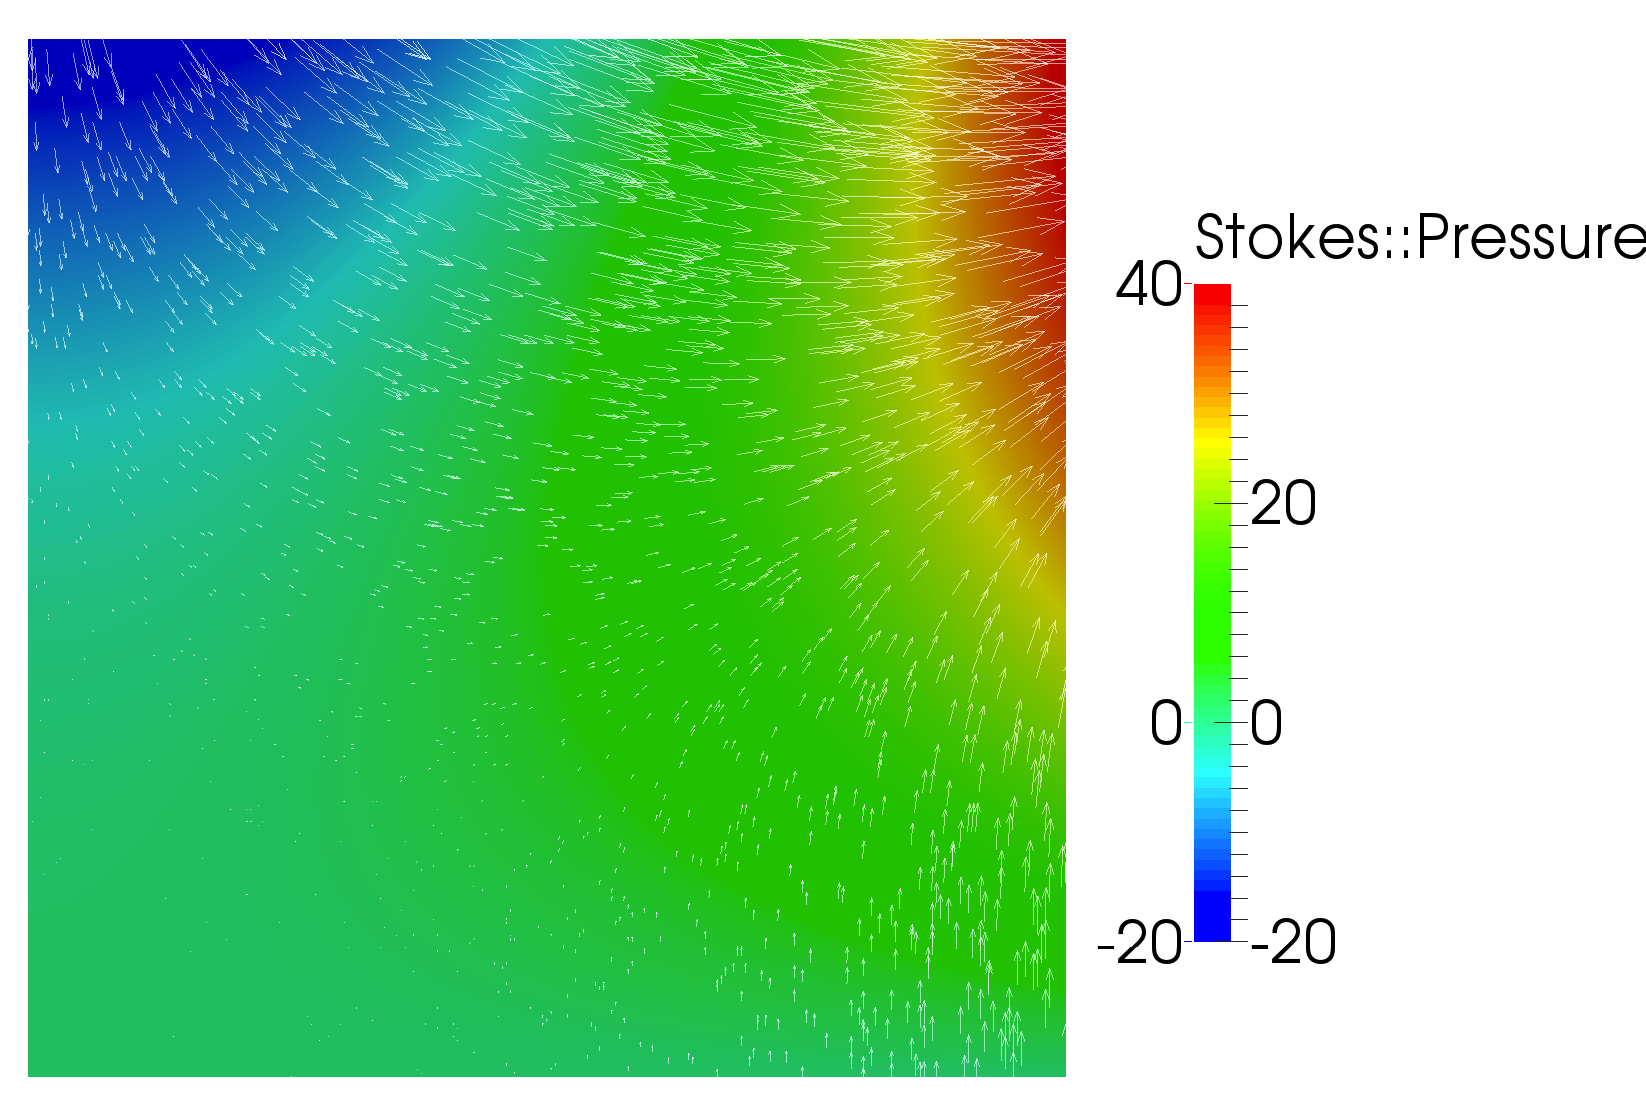
\includegraphics[width=.7\textwidth]{figures/stokes_flow.png}
  \caption{MMS solution of Stokes equation from
    \cite{elman_finite_2005} showing the pressure field in the background color map and the velocity field shown with arrows.}
  \label{fig:stokesMMS}
\end{figure}
and the convergence behavior is
\begin{figure}[htbp!]
  \centering
  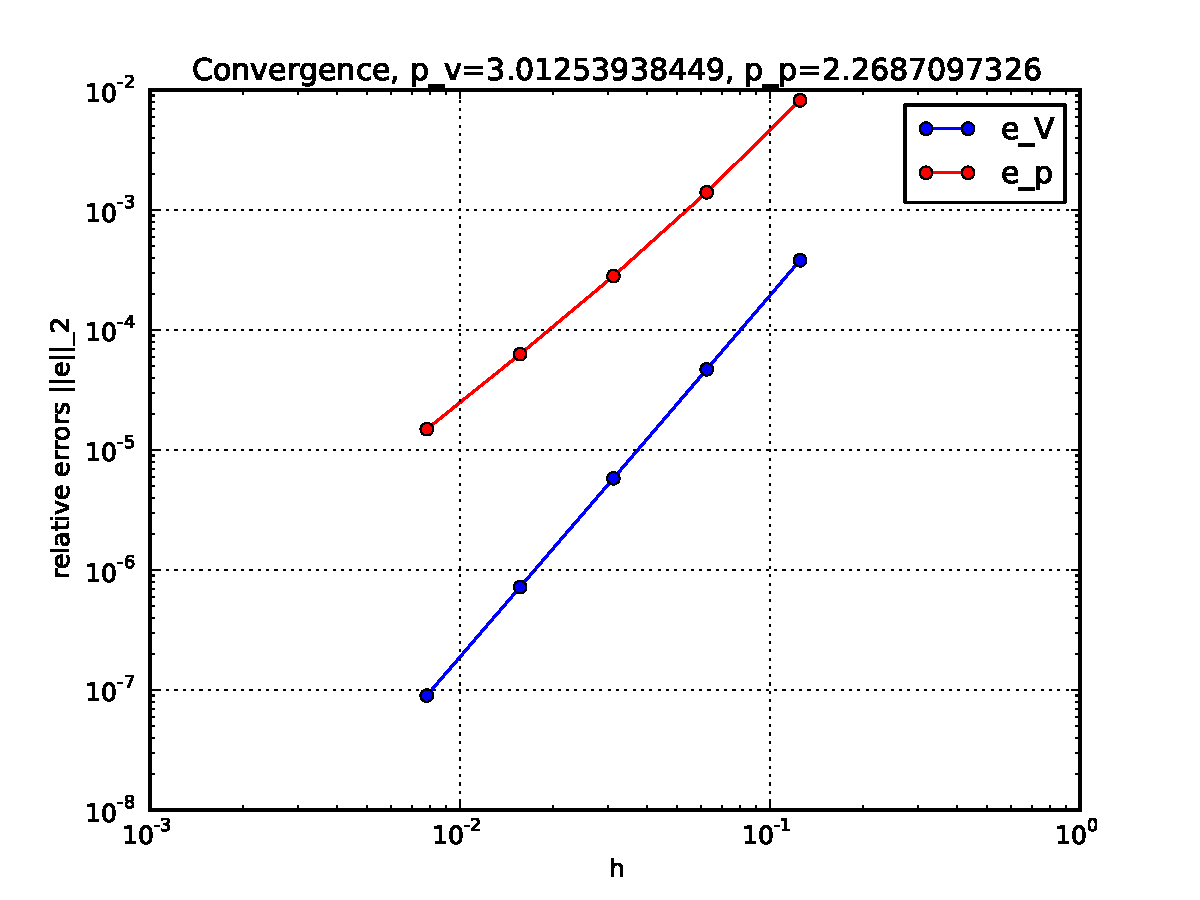
\includegraphics[width=.7\textwidth]{figures/Stokes_convergence.pdf}
  \caption{Convergence behavior of stokes solution for isoviscous stokes.}
  \label{fig:stokes_convergence}
\end{figure}
which shows larger errors for pressure which decrease as $h^{2}$
compared to errors for velocity which scale as $h^{3}$.


%% FIXME:  Give more detail on how to set this problem up



\section{Themes and Variations}
\label{sec:themes-variations}

\subsection{Iterative Solvers and Fieldsplit preconditioners}
\label{sec:iterative-solvers-1}

For moderate sized problems in 2-D, sparse-direct solvers can be quite
efficient and extremely robust methods.  However, for larger problems
and particularly in 3-D we need to move to iterative solvers.  There
is a large literature on iterative solvers for Stokes equation, 
%% FIXME and future versions of this tutorial will hopefully address
%% at least some of this. 
however, here we will just present the optimal method for isoviscous
stokes presented in \cite{elman_finite_2005} as a means of introducing
PETSc's fieldsplit block-preconditioners as implemented in \TF{}.

The discrete inner linear solve in a Newton iteration for Stokes can
be written
\begin{equation}
  \label{eq:21}
     \left[
\begin{array}{cc}
  K & G  \\
  G^{T} & 0 \\
  \end{array}
  \right]
  \left[
    \begin{array}{c}
      \delta \vec{v} \\
      \delta p \\
    \end{array}
  \right] = -\left[
    \begin{array}{c}
      F_{\vec{v}} \\
      F_{p}\\
    \end{array}
  \right]
\end{equation}


%%% Local Variables: 
%%% mode: latex
%%% TeX-master: "tftutorials"
%%% End: 
